The goal of this chapter is to give a description of the Bacco protocol and to discuss the
implementation choices that were made to deploy it. This is achieved using a top-down ordering for the level
of detail, meaning that the overview is presented before the specifics.

\section{Overview}
We will now describe a simple network that makes use of Bacco to better understand its operating principle. The
network is built upon 4 categories of devices:

\begin{description}[font=$\bullet$~\normalfont\scshape\color{blue!50!black}]
    \item [Sender node] - collects data and sends it to a Gateway or Repeater using Bacco over LoRa modulation;
    \item [Repeater node] - listens to incoming Bacco messages from Senders and forwards them to a Gateway;
    \item [Gateway node] - collects data coming from Sender or Repeater nodes and sends it to the web server. In the example
        shown in Figure \ref{img: network stack}, this is achieved using \gls{FTP} over a \gls{GSM} or \gls{LTE} mobile
        network. This node has the role of coordinating and synchronizing Sender nodes. It can be optionally configured
        to perform pre-processing operations (e.g. filtering, smoothing, interpolation ...) on the incoming data;
    \item [Web server] - receives data coming from the Gateways, elaborates it, and makes it available to the user. Note
        that the scheme of communication involving this device is not covered by Bacco.
\end{description}
\\
\begin{figure}[ht]
    \centering
    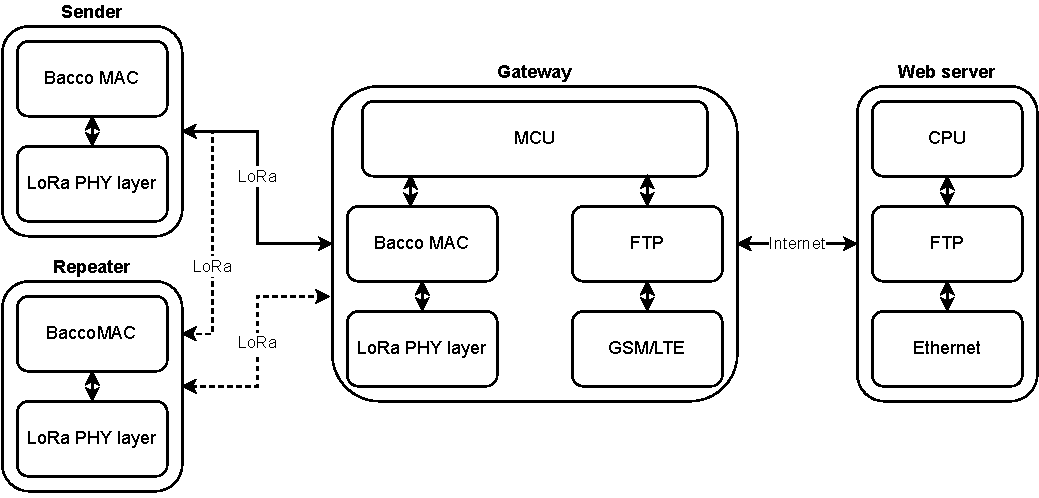
\includegraphics[width=1.0\textwidth]{uml/network_stack.pdf}
    \caption{Schematic representation of an example network using Bacco.}
    \label{img: network stack}
\end{figure}

\section{Topology}
The network has a star-of-stars topology, in which the zeroth level is occupied by the Web server, the first level by
Gateways and Repeaters, and the second level contains the Senders.
Figure \ref{network topology img} shows the types of devices that are involved and their communication scheme. \\
The structure is equivalent to a tree, hence we can define a hierarchy for the nodes. The root node is the central web server
and its children nodes are the Gateways. All sender nodes are children of either a Gateway or a Repeater and have no
children, so they correspond to the leaves of the tree.

\begin{figure}[ht]
    \centering
    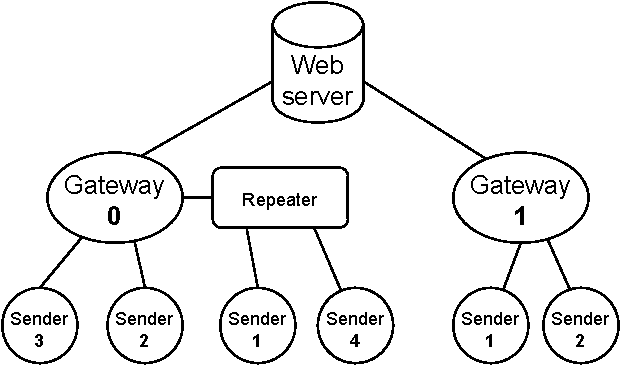
\includegraphics[width=1.0\linewidth]{uml/network_topology.pdf}
    \caption{Example network topology}
    \label{network topology img}
\end{figure}

\section{Addressing}
It is crucial to identify each Sender node to contextualize the messages coming to the Gateway node.
This is achieved by assigning them a unique identifier, represented by a natural number in the range $\[1,254\]$.
Address 0 is reserved for the Receiver and address 255 is used as a globally invalid address.
This limits the number of Sender nodes connected to a single Gateway to 254 \footnote{This choice is influenced
    by the considerations presented in Section \ref{subsec: regulations}}. If necessary, the network can scale up by using additional Gateways.
Note that since Repeaters do not produce messages themselves nor they modify the forwarded ones, they will not be
given an identifier.

\section{Interference Mitigation}
The LoRa PHY protocol specification does not fully cover the matter of sharing the communication link between multiple
devices, thus it is necessary to define methods for doing so, to minimize interference and achieve
a reliable exchange of information. Different techniques are applied in the domain of both time and frequency.

\subsection{Channel Activity Detection}
\Gls{CAD} is a feature available for most LoRa transcievers \cite{cad}. In this mode, the LoRa node
listens for any transmission on a specific frequency and, if it detects a signal, an interrupt is returned to the
\gls{MCU}. This
presents a possible \gls{CSMA} mechanism.\\
Bacco does not make use of \gls{CAD} for data packets, but it enables it in specific situations such as network discovery (discussed
in Section \ref{Network discovery}).

\subsection{IQ Inversion}
\Gls{IQ} inversion is a LoRa primitive that makes it possible to have 2 types of transmissions on the same frequency and
spreading factor, that are easily distinguishable for a receiver. The name \gls{IQ} usually refers to
signals that are out of phase from each other by $\frac{\pi}{4}$ rad. Despite that, LoRa uses the \gls{IQ} acronym to describe
signals with inverted chirp direction, namely up-chirp and down-chirp.\\
Bacco uses this technique to discriminate between uplink messages (i.e., from Sender to
Gateway/Repeater or from Repeater to Gateway) and downlink messages (i.e., from Gateway to Sender/Repeater or from
Repeater to Sender). This implies that Sender nodes and Gateway nodes are not able to communicate with other devices of
the same category (e.g. a Sender would not detect any transmission coming from a Sender).

%\begin{figure}[ht]
%\centering
%\begin{subfigure}[b]{0.45\linewidth}
%\begin{subfigure}[b]{\linewidth}
%\begin{tikzpicture}
%\begin{axis}[width=\linewidth, height=4cm, title={\textbf{Up-chirp}}, xlabel={Time [ms]}, ylabel={Amplitude [V]}]
%\addplot[color=red, samples=500][domain=0:1]{sin(x*x*5000)};
%\end{axis}
%\end{tikzpicture}
%\end{subfigure}
%\begin{subfigure}[b]{\linewidth}
%\begin{tikzpicture}
%\begin{axis}[width=\linewidth, height=4cm, title={\textbf{Down-chirp}}, xlabel={Time [ms]}, ylabel={Amplitude [V]}]
%\addplot[color=blue, samples=500][domain=0:1]{sin(5000*(1-x)*(1-x))};
%\end{axis}
%\end{tikzpicture}
%\end{subfigure}
%\end{subfigure}
%\hspace{0.08\linewidth}
%\begin{subfigure}[b]{0.45\linewidth}
%\begin{tikzpicture}
%\begin{axis}[width=\linewidth, height=8cm + \baselineskip, title={\textbf{Frequency plot}}, xlabel={Time
%[ms]}, ylabel={Frequency [Hz]}, ytick={0, 0.5, 1}, yticklabels={$F_0-\frac{B}{2}$, $F_0$, $F_0+\frac{B}
%{2}$}, legend entries={Down-chirp, Up-chirp}]
%\addplot[line width=0.5mm, color=blue, samples=500][domain=0:1]{1-x};
%\addplot[line width=0.5mm, color=red, samples=500][domain=0:1]{x};
%\end{axis}
%\end{tikzpicture}
%\end{subfigure}
%\caption{IQ inversion.}
%\label{img: iq inversion}
%\end{figure}

\subsection{Subnetting}
The LoRa protocol supports a wide range of carrier frequencies in the \gls{VHF} spectrum \footnote{For reference, the
SX1262\cite{sx1262} transceiver features a continuous frequency coverage from 150 MHz to 960 MHz}.\\
Bacco exploits this fact to build sub-networks that operate at different frequencies to achieve very low
interference between them. The set of used frequencies is defined by Equation \ref{set of frequencies}.
\begin{equation}
    \label{set of frequencies}
    f = \left\{ f_k : f_k = 868\text{MHz} + k \times 125\text{KHz}, k\in \left\{0...10 \right\} \right\}
\end{equation}
The main sub-network operates at the base frequency of 868.0 MHz, obtained by setting $k=0$ in Equation \ref{set of
frequencies}; it is composed of the Gateway and all the
Sender nodes connected to it. Every other sub-network operates at a different frequency that is obtained by choosing $k
\in \left\{1...10 \right\}$; they are composed of a Repeater and all the Sender nodes connected to it.
To be able to communicate with the Gateway, Repeaters need to forward the messages at the base frequency of the Gateway,
regardless of their operating frequency inside the sub-net.\\
A network using Bacco can have up to 10 Repeaters operating at different frequencies, however, if more coverage
is needed, it is possible to have multiple Repeater nodes working at the same frequency, given that they are not in
reach with each other. This is very important because of bouncing, a phenomenon that occurs when a message is sent
back and forth between Repeaters.\\
Figure \ref{repeaters subnet} shows a network consisting of 3 different sub-networks, represented with different colors;
the main one is in white, the blue one has a value of $k=2$, and the red one has a value of $k=1$.


\begin{figure}[ht]
    \centering
    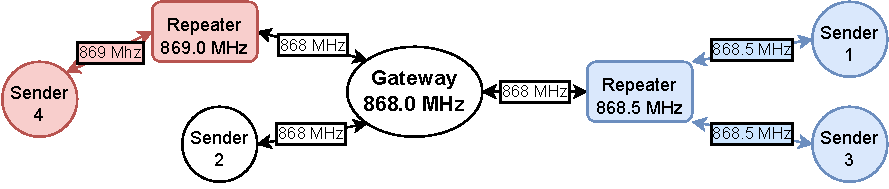
\includegraphics[width=\linewidth]{uml/repeaters_subnet.pdf}
    \caption{Example network with subnets in different colors.}
    \label{repeaters subnet}
\end{figure}


\subsection{Distribution Of Transmission Activity}
The Bacco protocol distributes activity on the radio channel over time with defined frames reserved for each Sender,
using an approach that was first introduced by the AlohaNet \cite{alohanet} protocol. Frames are equally distributed
between the maximum number of Senders that can be connected to a Gateway (i.e., $N_{max} = 254$), and the frame
assignment is based on the identifier (e.g. Sender1 to slot 1, Sender2 to slot 2, etc.). A Sender can only transmit
during its assigned frame, otherwise, the Gateway will send a time-correction message. (see Subsection \ref{clock drift
compensation} for a detailed explanation). The time delay between consecutive transmissions from the same Sender is a
constant value and it is called $C$ (cycle time). Between each frame, a time equivalent to $\frac{1}{3}$ of a Sender
frame is left as tolerance and is called a radio silence frame. At the end of a cycle, a time equal to $\frac{C}{5}$ is
reserved for the Gateway to upload the collected data. Figure \ref{timing diagram case 1} shows a schematic
representation of the time management used by Bacco. The cycle time is a user-defined parameter, and all the other
values are calculated based on it as shown in Table \ref{timing table}.\\

\begin{table}[ht]
    \caption{Time parameters calculation.}
    \label{timing table}
    \centering
    \setlength{\extrarowheight}{7pt}
    \begin{tabular}{ |c|c| }
        \hline
        \textbf{Parameter} & \textbf{Value}\\
        \hline
        Gateway frame time & $0.2 \cdot C$\\
        Sender frame time & $\frac{0.6 \cdot C}{N_{max}}$\\
        Silence frame time & $\frac{0.2 \cdot C}{N_{max}}$\\
        \hline
    \end{tabular}
\end{table}

\begin{figure}[ht]
    \centering
    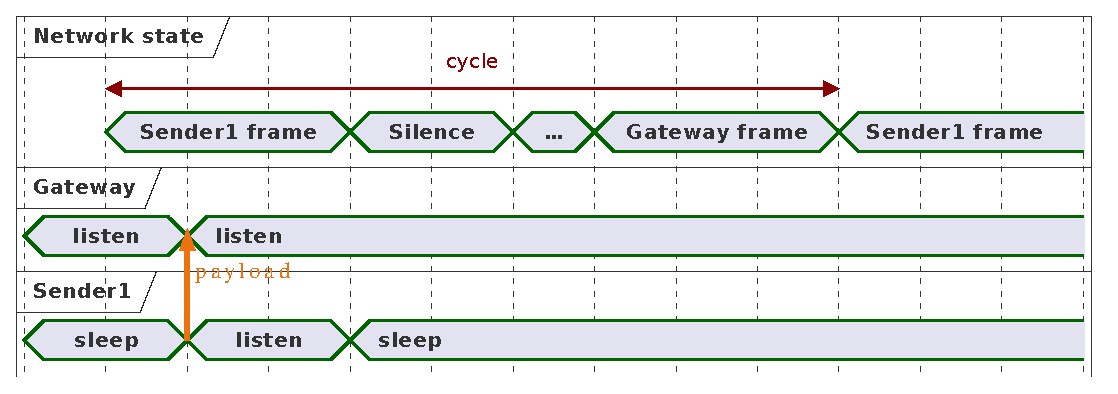
\includegraphics[width=1.0\textwidth]{uml/timings_case1.pdf}
    \caption{Timing diagram - Sender1 is in sync.}
    \label{timing diagram case 1}
\end{figure}

\subsubsection{Clock drift compensation}
\label{clock drift compensation}
All the Senders in the network need to transmit during their assigned frame; this means
that all the clocks of the devices are required to be in sync. This is hard to achieve without dynamic recalibration
because commercial oscillators can not provide a constant frequency source due to manufacturing imprecisions,
temperature gradient, etc...\\
To deal with this problem, Bacco assigns the Gateway node the role of coordinating the network timings through
the dispatch of downlink messages containing the network timestamp. Such a message
is sent as soon as the Gateway receives an uplink message that exceeds its correct time frame. Figure \ref{timing
diagram case 2} shows this specific case. In addition to that, the Gateway sends at least 1 downlink message every 10
uplink messages from the same Sender, to indicate that the connection is still active.

\begin{figure}[ht]
    \centering
    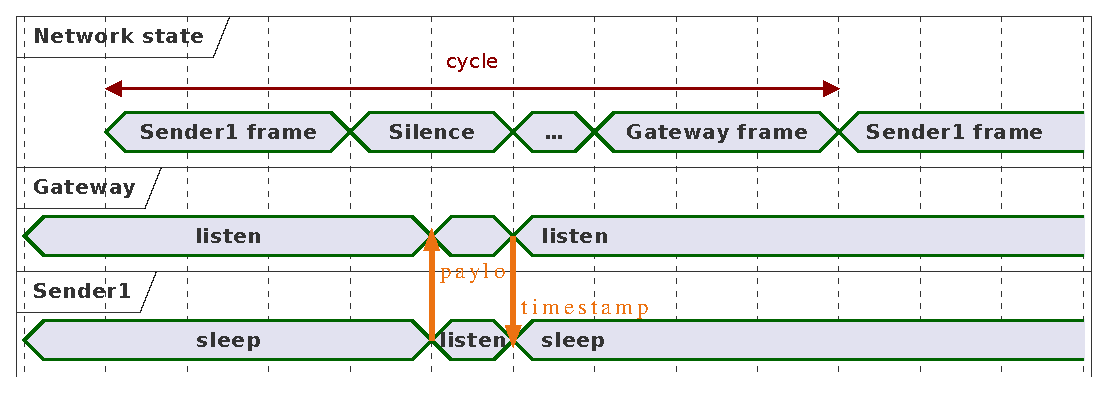
\includegraphics[width=1.0\textwidth]{uml/timings_case2.pdf}
    \caption{Timing diagram - Sender1 is out of sync.}
    \label{timing diagram case 2}
\end{figure}

\section{Network Discovery}
\label{Network discovery}
When a Sender node is first started, it needs to decide at what frequency to operate for minimizing the power
needed to reach a Repeater or Gateway. To this end, Bacco introduces Algorithm \ref{algo: network discovery}
for scanning nearby devices and selecting the most suitable. The Sender tries to establish communication with Repeaters and
Gateways throughout all the available frequencies by sending a particular type of message that triggers a \gls{SYN/ACK}
response. \Gls{CAD} will be used by the Sender to not interfere with ongoing communications; this is because the board does
not yet have an allocated time frame and thus can not decide when to transmit otherwise.

\begin{algorithm}[ht]
    \caption{Network discovery.}
    \label{algo: network discovery}
    \begin{algorithmic}

        \State rssi\_values $\gets$ $\[0,0,0,0,0,0,0,0,0,0\]$

        \While{all rssi\_values are equal to 0}
        \For{$k$ from 0 to 10}
        \State $f_k$ $\gets$ $868 \times 10^6 + k \times 125 * 10^3$
        \For{$i$ from 0 to 10}
        \Do
        \State sleep for 1 s
        \State enter CAD mode at frequency $f_k$ for 1.5 s
        \doWhile{activity detected by CAD}
        \State send sensing message
        \State enter receive mode for 3 s
        \If{received SYN/ACK}
        \State $\text{rssi}\_values\[k\]$ $\gets$ current rssi
        \State \textbf{break}
        \EndIf
        \EndFor
        \EndFor
        \EndWhile
        \State \Return $868 \times 10^6 + \text{argmin(rssi\_values)} \times  125 * 10^3$
    \end{algorithmic}
\end{algorithm}


\section{Network Joining}
When a Sender node needs to connect to the network for the first time, it does not yet have an identifier nor its clock
is in sync. The procedure to achieve that will be called the joining process. Note that we assume that the
Sender node has already selected the frequency of operation, as described in section \ref{Network discovery}.\\
We will ignore the act of forwarding made by any optional Repeater node, as in this case it does not affect the
content of the messages, but note that delay and error rate would raise in that situation. All the messages sent from Sender
and Receiver make use of \gls{CAD} to make sure the channel is free before the actual transmission; this step will be omitted
in the description for brevity. First, the Sender transmits a \gls{SYN} to the Gateway and waits for a \gls{SYN/ACK}
response for 3 s. If no message is received, another \gls{SYN} is sent a maximum of 10 times. After that,
the Gateway waits for 3 s for an \gls{ACK} from the Receiver, and if no message is received it will try again
for a maximum of 10 times. The \gls{SYN/ACK} contains the timestamp of the network as well as the assigned identifier.
If the maximum number of iterations is reached in any of the steps, the process starts again after 30 minutes.
Figure \ref{img: network joining} shows a schematic representation of the process.

\begin{figure}[ht]
    \centering
    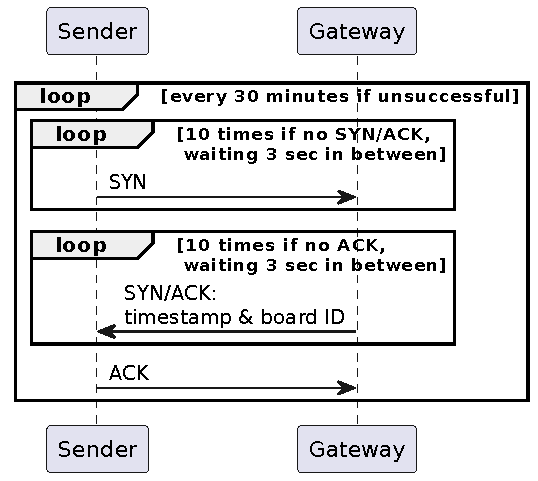
\includegraphics[width=200pt]{uml/network_joining.pdf}
    \caption{Network joining process.}
    \label{img: network joining}
\end{figure}

\section{Downlink Commands}
In some situations such as transmission power adaption, it is required to be able to change the behavior of the
network dynamically and reliably. Bacco achieves this by exchanging specialized packets that contain
commands. Each message contains a command and needs to be acknowledged by the Sender to the Gateway/Repeater in a similar way as done during the
network joining procedure. Figure \ref{img: command ack} shows a graphical representation of the process.\\
The following commands are defined by the protocol, and each of them is associated with an opcode as shown in Table
\ref{tab: opcodes}:
\begin{description}[font=$\bullet$~\normalfont\scshape\color{blue!50!black}]
    \item [Shutdown] - If this command is sent and processed successfully, the Sender goes to deep sleep indefinitely until a
        manual reset is invoked by pressing a physical button;
    \item [Enter sleep mode] - If this command is processed successfully, the Sender stops sending data, but it keeps
        listening for incoming messages/commands during its time frame;
    \item [Wakeup] - If this command is processed successfully, the Sender enters normal/active mode
        and thus starts to transmit data;
    \item [Increase transmission power] - If this command is processed successfully, the Sender increases its
        transmission power by $P_{step}= 3 \text{ dBm}$;
    \item [Decrease transmission power] - If this command is processed successfully, the Sender decreases its
        transmission power by $P_{step}= 3 \text{ dBm}$.
\end{description}
\\
\begin{table}[ht]
    \caption{Table of opcodes.}
    \label{tab: opcodes}
    \centering
    %\setlength{\extrarowheight}{5pt}
    \begin{tabular}{ |c|c| }
        \hline
        \textbf{Command} & \textbf{Opcode as 7 bit unsigned integer}\\
        \hline
        Shutdown & 0\\
        \hline
        Enter sleep mode & 1\\
        \hline
        Wakeup & 2\\
        \hline
        Increase transmission power & 3\\
        \hline
        Decrease transmission power & 4\\
        \hline
        Reserved for later use & [4, 50]\\
        \hline
        User-defined & [51, 127]\\
        \hline
    \end{tabular}
\end{table}

\begin{figure}[ht]
    \centering
    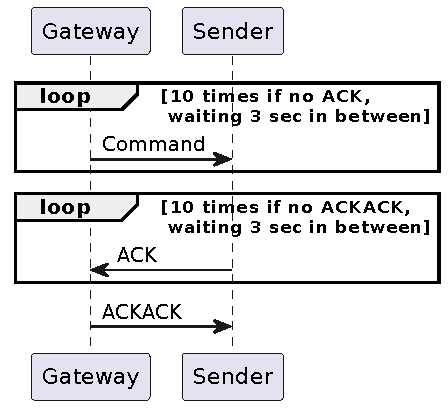
\includegraphics[width=200pt]{uml/command_ack.pdf}
    \caption{Command sending process.}
    \label{img: command ack}
\end{figure}

\section{Transmission Power Adaption}
\label{sec: transmission power adaption}
Since Senders can be placed at different distances from a Gateway or Repeater, it is useful to optimize the power
used by the node to transmit. The default value for the transmission power is equal to $P_{0}$; starting from that, the
network will automatically drift towards a more suitable value according to the following triggers and Table \ref{tab:
TX adaption parameters}:
\begin{itemize}
    \item If a Sender has not received any downlink messages during
        the last 20 frames, then its transmission power will be increased by $P_{step}$ up to a maximum of $P_{max}$
    \item If 10 out of the last 10 messages received by a Repeater or a Gateway from the same Sender
        satisfy $\text{RSSI} > \text{RSSI}_{high}$ and $\text{SNR} > \text{SNR}_{high}$, then
        a command is sent telling to decrease the transmission power by $P_{step}$ down to a minimum of
        $P_{min}$
    \item If 8 out of the last 10 messages received by a Repeater or a Gateway from the same Sender
        satisfy $\text{RSSI} < \text{RSSI}_{low}$ or have not been received, then a command is sent telling to
        increase the transmission power by $P_{step}$.
\end{itemize}
\\
\begin{table}[ht]
    \caption{Parameters for transmit power adaption algorithm.}
    \label{tab: TX adaption parameters}
    \centering
    %\setlength{\extrarowheight}{5pt}
    \begin{tabular}{ |c|c| }
        \hline
        \textbf{Parameter} & \textbf{Value}\\
        \hline
        $P_{0} = P_{max}$ & 14 dBm\\
        \hline
        $P_{min}$ & 5 dBm\\
        \hline
        P$_{step}$ & 3 dBm\\
        \hline
        RSSI$_{low}$ & -115 dBm\\
        \hline
        RSSI$_{high}$ & -60 dBm\\
        \hline
        SNR$_{low}$ & -7 dBm\\
        \hline
    \end{tabular}
\end{table}
Gateways and Repeaters always operate at $P_{0}$, since power efficiency is less critical than ensuring the highest
possible delivery rate.


\section{Packet Format}
In this section, the bit format of the messages is shown. The analysis will be split between uplink packets and downlink
packets.

\subsection{Uplink Packet Format}
\label{sec: uplink packet format}
Uplink messages are sent from a Sender to a Gateway/Repeater or from a Repeater to a Gateway. It has a variable
length and it is transmitted using up-chirps, i.e., with \gls{IQ} inversion disabled. The least significant byte
contains the Sender's identifier represented as an 8-bit unsigned integer. The second least significant byte contains
the size of the payload in bytes as an 8-bit unsigned integer. The rest of the message contains the payload and has a
length defined by the previous field. Figure \ref{img: uplink packet format} shows the packet format.

\begin{figure}[ht]
    \centering
    \begin{bytefield}[bitwidth=1em]{32}
        \bitheader{0,8,16} \\
        \bitbox{8}{Sender ID} & \bitbox{8}{Payload size}
                              & \bitbox{16}{Payload}\\
                              \bitbox[t]{16}{$\underbrace{\hspace{16em}}_{\text{\normalsize Header}}$}
    \end{bytefield}
    \caption{Uplink packet format.}
    \label{img: uplink packet format}
\end{figure}


\subsection{Downlink Packet Format}
\label{sec: downlink packet format}
Downlink messages are sent from a Gateway to a Sender/Repeater or from a Repeater to a Sender. It has a fixed
length of 5 bytes and it is transmitted using down-chirps, i.e., with \gls{IQ} inversion enabled. The least significant
byte contains the identifier of the Sender for which the message is directed as an 8-bit unsigned integer. The
following bit contains the type of the message: 0 represents a time sync message whereas 1 represents a command
message. The content of the following bits depend on the type of message: in the case of a time sync message, the
remaining 31 bits contain the timestamp, whereas in the case of a command message, the first 7 bits contain an opcode and
the remaining 14 bits are left for padding and can be later used by future revisions of the protocol. Figure \ref{img:
downlink packet format}, \ref{img: downlink timestamp packet format}, \ref{img: downlink command packet format} show the
general format, the timestamp format, and the command format respectively.

\vspace{1cm}
\newcommand{\bitlabel}[2]{%
    \bitbox[]{#1}{%
        \raisebox{0pt}[4ex][0pt]{%
            \turnbox{45}{\fontsize{9}{9}\selectfont#2}%
        }%
    }%
}
\begin{figure}[H]
    \centering
    \begin{bytefield}[]{40}
        \bitlabel{8}{} & \bitlabel{1}{Message type} & \bitlabel{31}{}\\
        \bitheader{0,8,9,39} \\
        \bitbox{8}{Sender ID} & \bitbox{1}{}
                              & \bitbox{31}{$\cdots$}
    \end{bytefield}
    \caption{Downlink packet format.}
    \label{img: downlink packet format}
\end{figure}

\begin{figure}[H]
    \centering
    \begin{bytefield}[]{40}
        \bitheader{0,8,9,39} \\
        \bitbox{8}{Sender ID} & \bitbox{1}{0}
                              & \bitbox{31}{Timestamp}
    \end{bytefield}
    \caption{Downlink packet format for timestamps.}
    \label{img: downlink timestamp packet format}
\end{figure}

\begin{figure}[H]
    \centering
    \begin{bytefield}[]{40}
        \bitheader{0,8,9,16,39} \\
        \bitbox{8}{Sender ID} & \bitbox{1}{1}
                              & \bitbox{7}{Opcode}
                              & \bitbox{24}{Padding/later use}
    \end{bytefield}
    \caption{Downlink packet format for commands.}
    \label{img: downlink command packet format}
\end{figure}

\subsection{Comparing Bacco And LoRaWAN Packet Formats}
We will now compare Bacco's packet format to LoRaWAN's. The latter is described thoroughly by Semtech's official
documentation
\cite{lorawan_packets}, a schematic reference can be found in
Figure \ref{img: lorawan uplink format} and \ref{img: lorawan downlink format}.\\
The focus of the comparison will be on the total size of the packets rather than the function of each field, to analyze
the overhead associated with each protocol.

\begin{figure}[ht]
    \centering
    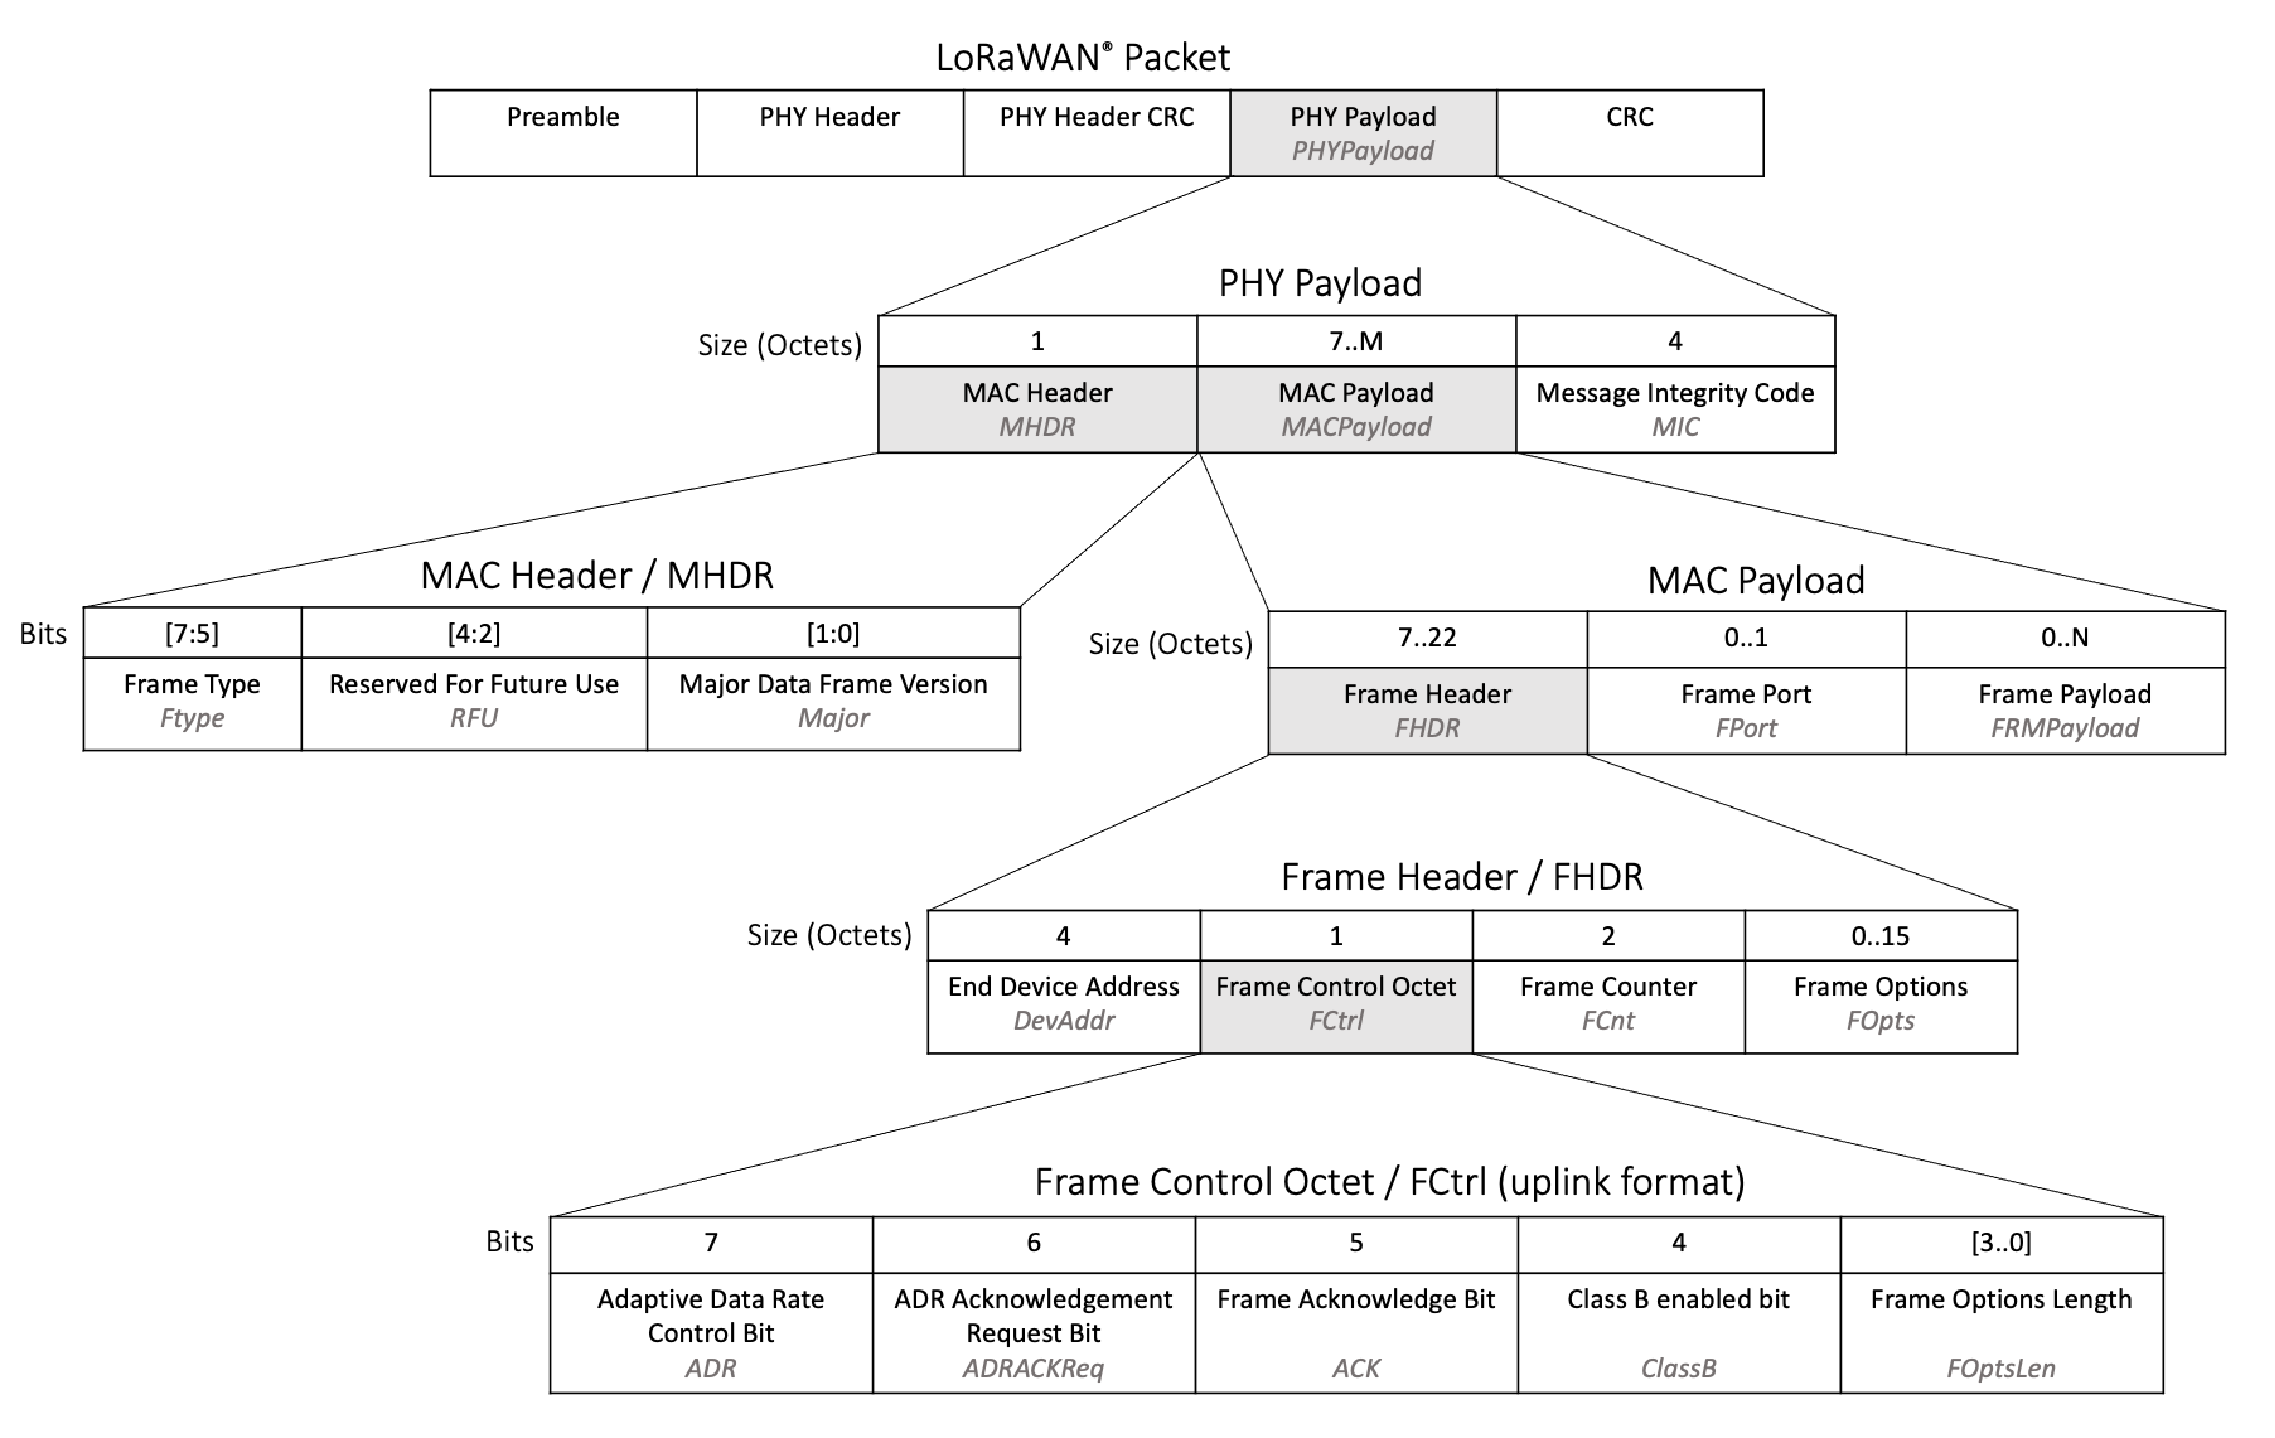
\includegraphics[width=1.0\textwidth, trim={0 0 0 125pt}, clip]{uml/lorawan_uplink_format.pdf}
    \caption{LoRaWAN uplink packet format.}
    \label{img: lorawan uplink format}
\end{figure}

\begin{figure}[ht]
    \centering
    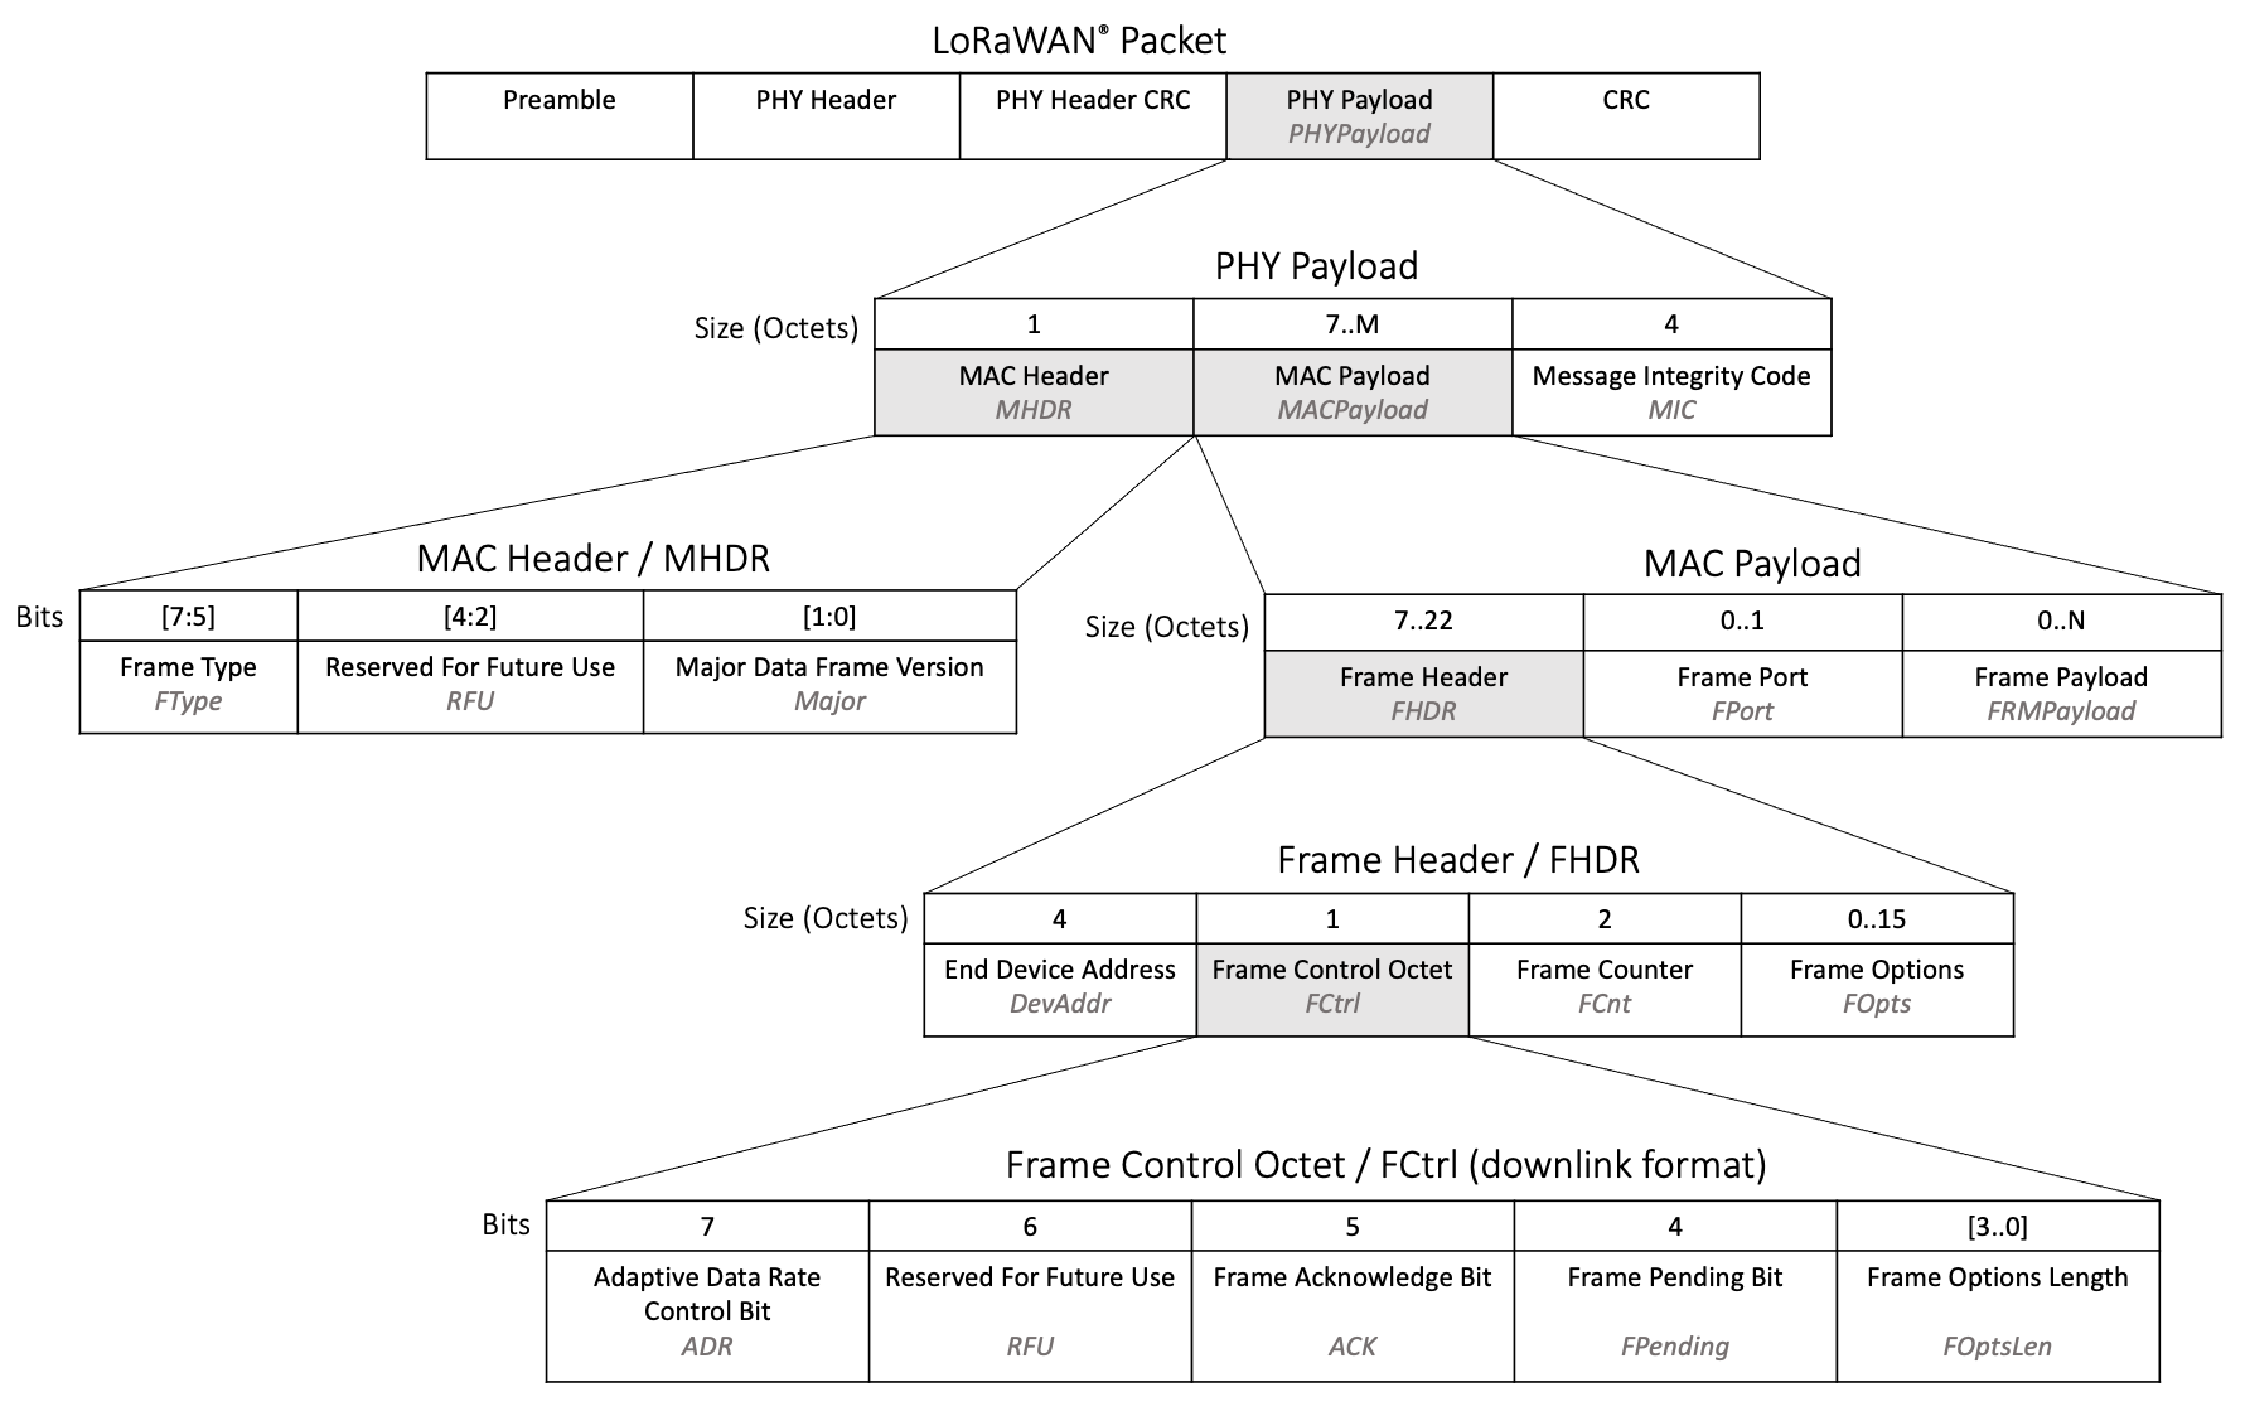
\includegraphics[width=1.0\textwidth, trim={0 0 0 115pt}, clip]{uml/lorawan_downlink_format.pdf}
    \caption{LoRaWAN downlink packet format.}
    \label{img: lorawan downlink format}
\end{figure}

\subsubsection{Uplink Packets}
\label{subsec: bacco and lorawan uplink packet format}
Considering two uplink packets containing the same payload and transmitted with the two protocols under
analysis, we can observe that Bacco uplink packets feature a fixed header size of 2 bytes as described in Section \ref{sec:
uplink packet format}, while LoRaWAN uses a MAC header size that varies between 7 and 23 bytes.\\
To show that, we can consider an empty \textit{Frame Payload} and sum all the other
fields' sizes to get the overall header size. LoRaWAN supports a range of sizes for the uplink packets; the lower bound
is given by Frame Header: 7 + Frame Port: 0; the upper bound is given by Frame Header: 22 + Frame Port: 1. This means
that, at a fixed payload size, Bacco uplink packets are always shorter by a constant factor between 5 and 21 bytes.
Figure \ref{img: uplink packet size} shows a plot of the total size of an uplink packet compared to its payload lenght,
using both Bacco and LoRaWAN.

\begin{figure}[ht]
    \centering
    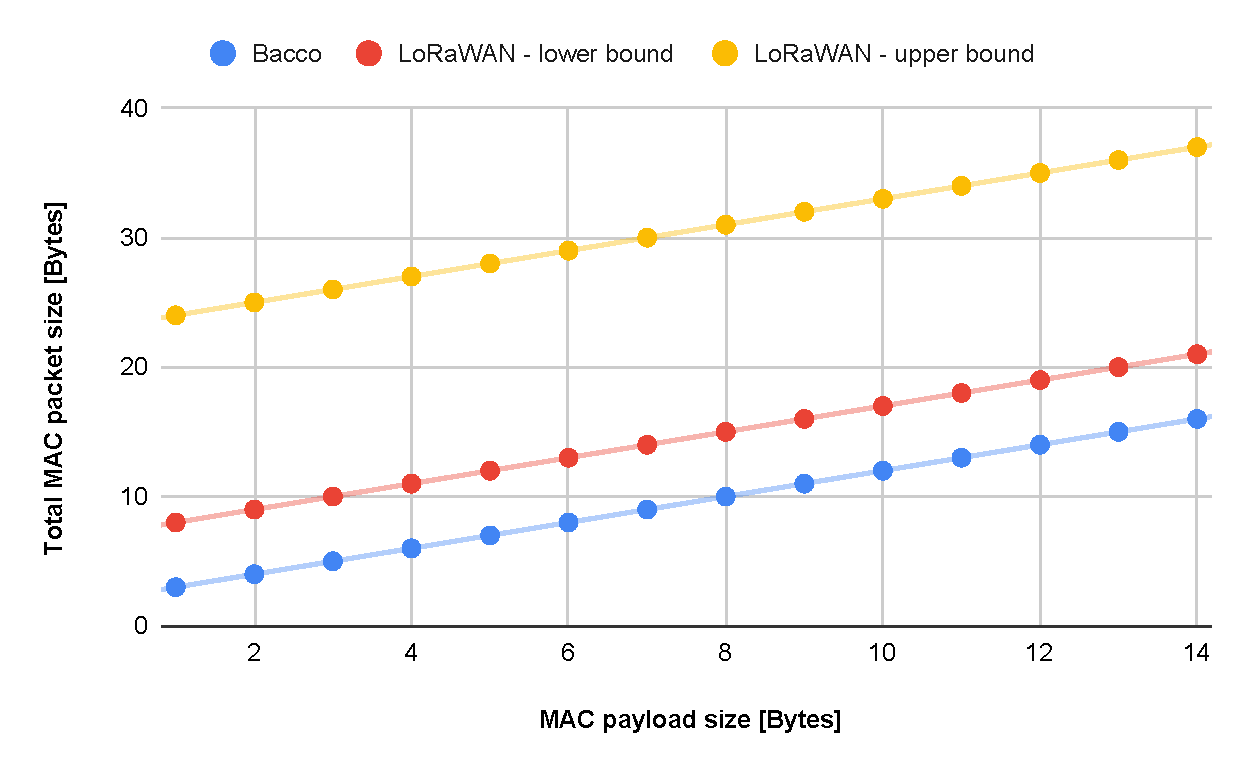
\includegraphics[width=1.0\textwidth]{images/uplink_packet_size.pdf}
    \caption{LoRa and Bacco total packet size with respect to payload size}
    \label{img: uplink packet size}
\end{figure}


\subsubsection{Downlink Packets}
Considering two uplink packets containing the same payload, but trasmitted using the two protocols under analysis, we
can observe that Bacco downlink packets feature a fixed overall size of 5 bytes as discussed in Section \ref{sec:
downlink packet format}, while LoRaWAN uses packets with a header of size between 7 and 23 bytes (the
calculation is analogous to the one of the uplink case, discussed in Section \ref{subsec: bacco and lorawan uplink
packet format}).
